\section{Method}
\label{sec:method}

\begin{figure*}[t]
\vskip 0.2in
    \centering
    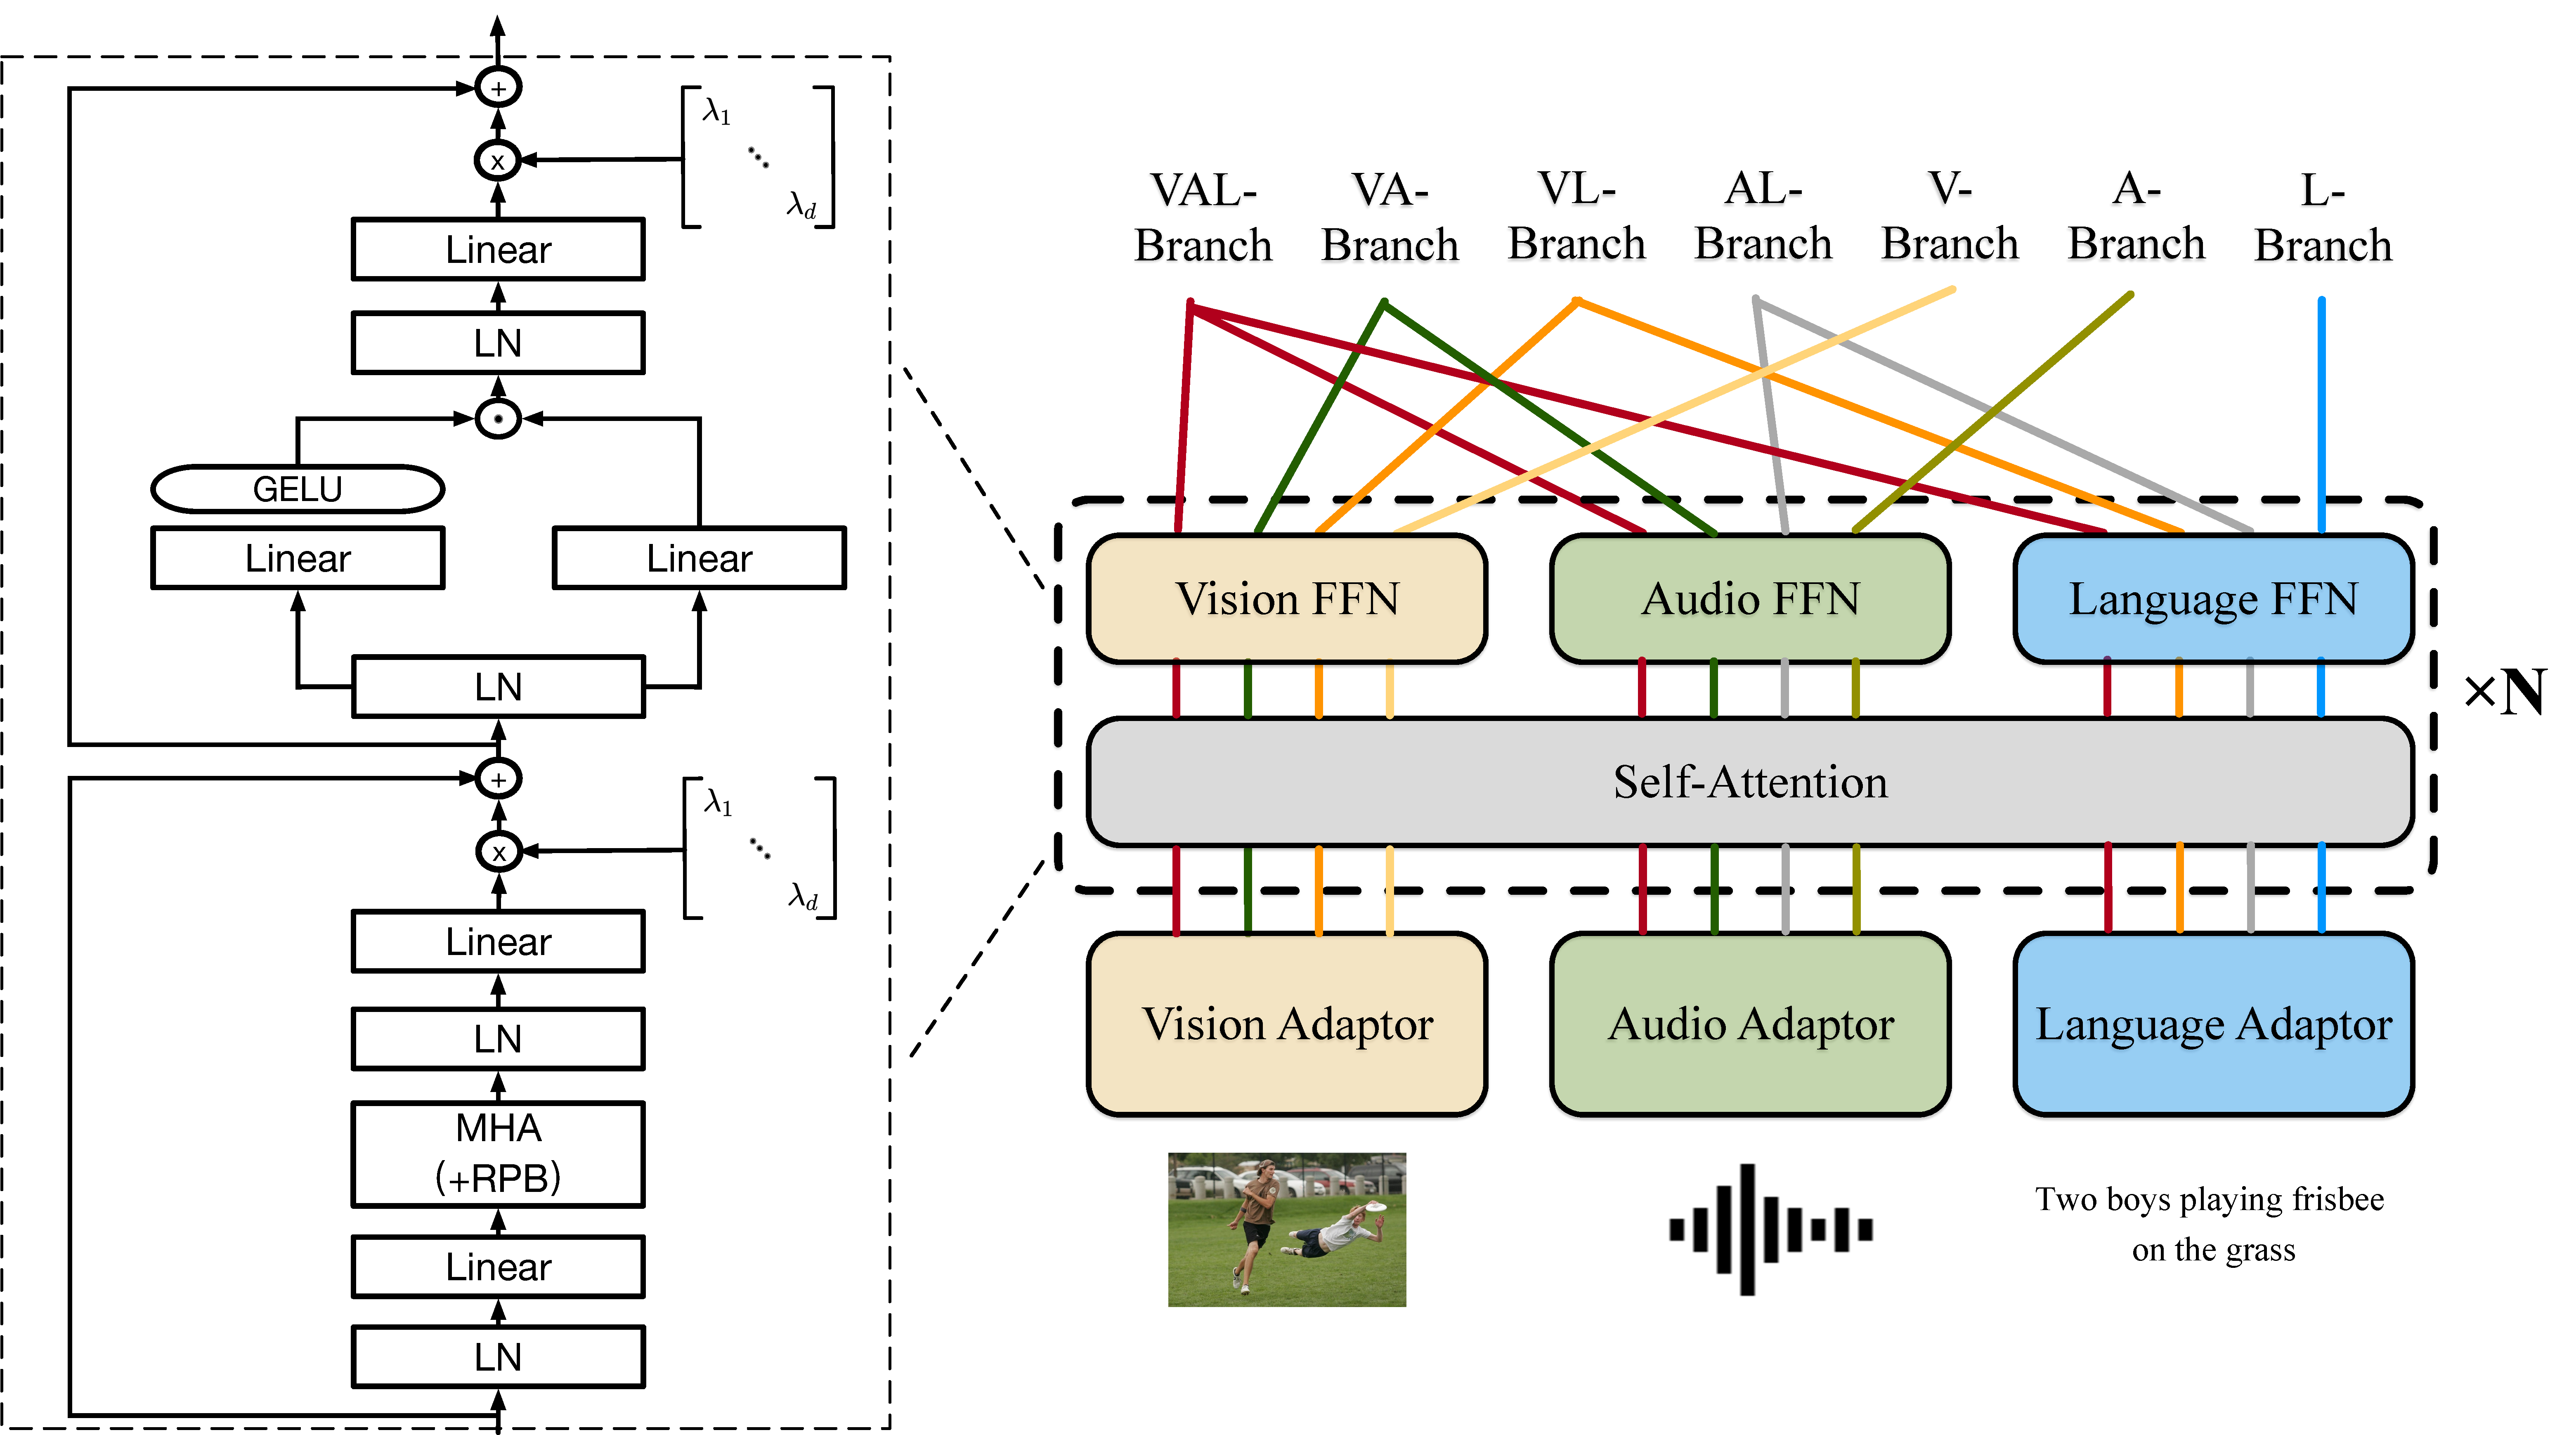
\includegraphics[width=0.85\linewidth]{pic/model_new2.pdf}
    \caption{\textbf{The architecture of \onepeace}. 
    % It consists of multiple modules that are specific to each modality (e.g., vision adapter) as well as modules that are shared across modalities (e.g., self-attention layer). 
    It consists of three modality adapters and a modality fusion encoder.
    \onepeace can be disassembled into different branches to handle different tasks.
    For example, the vision adapter, self-attention layers, and vision FFNs can be combined into V-Branch to handle vision tasks.}
    \label{fig:model}
\end{figure*}

\subsection{Architecture}
The model architecture of \onepeace consists of three modality adapters and a modality fusion encoder.
The overall architecture is shown in Figure~\ref{fig:model}.

\paragraph{Modality Adapters.}
We design modality adapters to convert different raw signals into unified features.
Note that these adapters do not interact with each other, which affords us the flexibility to choose appropriate networks for them, such as Transformers~\cite{transformer,vit,swin}, CNNs~\cite{mnist,resnet}, RNNs~\cite{rnn,gru}, etc.
We design three lightweight modality adapters for \onepeace:

\begin{itemize}
    \item \textbf{Vision Adapter (V-Adapter).} Given an image, we use a hierarchical MLP (hMLP) stem~\cite{Touvron2022ThreeTE} to patchify the image by gradually increasing the patch size to $16 \times 16$. There is no interaction between different patches. Then the image patches are flattened into a sequence and prepended with a vision class embedding. By adding the absolute positional embeddings into the image embeddings, the image representation is $E^V=\langle \bm{e}^V_{cls}, \bm{e}^V_{1}, \bm{e}^V_{2}, ..., \bm{e}^V_{M} \rangle$, where $M$ denotes the total number of image patches.
    \item \textbf{Audio Adapter (A-Adapter).} Given an audio, we set the sample rate to 16kHz and normalize the raw audio waveform to zero mean and unit variance. Then the normalized waveform is processed by a convolutional feature extractor~\cite{wav2vec2} to get the audio embeddings. Instead of using the absolute positional embeddings, we use a convolution layer to extract relative position information and add it to the audio embeddings~\cite{Mohamed2019TransformersWC}. With a prepended audio class embedding, we obtain the audio representation $E^A=\langle \bm{e}^A_{cls}, \bm{e}^A_{1}, \bm{e}^A_{2}, ..., \bm{e}^A_{N} \rangle$, where $N$ denotes the length of the audio representation.
    \item \textbf{Language Adapter (L-Adapter).} Given a text, we first apply byte-pair encoding (BPE) \cite{bpe} to transform it to a subword sequence. Two special tokens $\left[{\rm CLS}\right]$ and $\left[{\rm EOS}\right]$ are inserted at the beginning and end of the sentence to indicate its start and end. Then an embedding layer is used to embed the subword sequence to the text embeddings. After summing the text embeddings with absolute positional embeddings, we obtain the text representation $E^L=\langle \bm{e}^L_{cls}, \bm{e}^L_{1}, \bm{e}^L_{2}, ..., \bm{e}^L_{K}, \bm{e}^L_{eos} \rangle$, where $K$ denotes the text sequence length.
\end{itemize}

\paragraph{Modality Fusion Encoder.} 
Following previous works~\cite{simvlm,ofa,coca,beit3,ofasys}, the modality fusion encoder is based on the Transformer architecture~\cite{transformer}. 
We set up a shared self-attention layer and three modality feed-forward networks (FFNs) in each Transformer block.
The shared self-attention layer enables the interaction between different modalities through the attention mechanism.
The three modality FFNs (V-FFN, A-FFN, and L-FFN) can further extract information within their respective modalities.
To stabilize training and enhance model performance, we make the following improvements:

\begin{itemize}
    \item \textbf{Sub-LayerNorm.} We incorporate Sub-LayerNorm~\cite{magneto} into each Transformer block to enhance training stability. Specifically, We insert layer normalization before the input projection and output projection of each self-attention layer and FFN layer. In our preliminary experiments, we find that Sub-LayerNorm can achieve better performance compared to the Pre-LayerNorm~\cite{gpt3}.
    \item \textbf{GeGLU Activation Function.} To further improve performance, we replace the activation function in FFN with GeGLU~\cite{glu} activation function. The intermediate dimension of FFN is set to $4$ times the embedding dimension, which is consistent with the practice of PaLM~\cite{palm}.
    \item \textbf{Relative Position Bias (RPB).} For positional information, we introduce 1D relative position bias~\cite{T5} for text and audio, and 2D relative position bias for image~\cite{coatnet}. At the pretraining stage, the relative position bias of different self-attention layers is shared. At the fine-tuning stage, we decouple the relative position bias of each self-attention layer and let them inherit the weights of the pretrained relative bias.
    \item \textbf{LayerScale.} We use LayerScale~\cite{cait} to dynamically adjust the output of each residual block. Specifically, before adding to the residual, we multiply the output of each layer (e.g., self-attention layer and FFN) by a learnable diagonal matrix, whose values will be initialized to $1e-6$. In our preliminary experiments, LayerScale is beneficial for stabilizing training and improving performance.
\end{itemize}

This "sharing-separated" architecture enables \onepeace to disassemble into different branches that handle tasks for various modalities.
For example, the vision adapter, self-attention layer, and vision FFNs can be combined into the vision branch (V-Branch) to process vision tasks.
Similarly, we named other branches as audio branch (A-Branch), language branch (L-Branch), vision-audio branch (VA-Branch), vision-language branch (VL-Branch), audio-language branch (AL-Branch), and vision-audio-language branch (VAL-Branch).

\begin{figure*}[t]
\vskip 0.2in
    \centering
    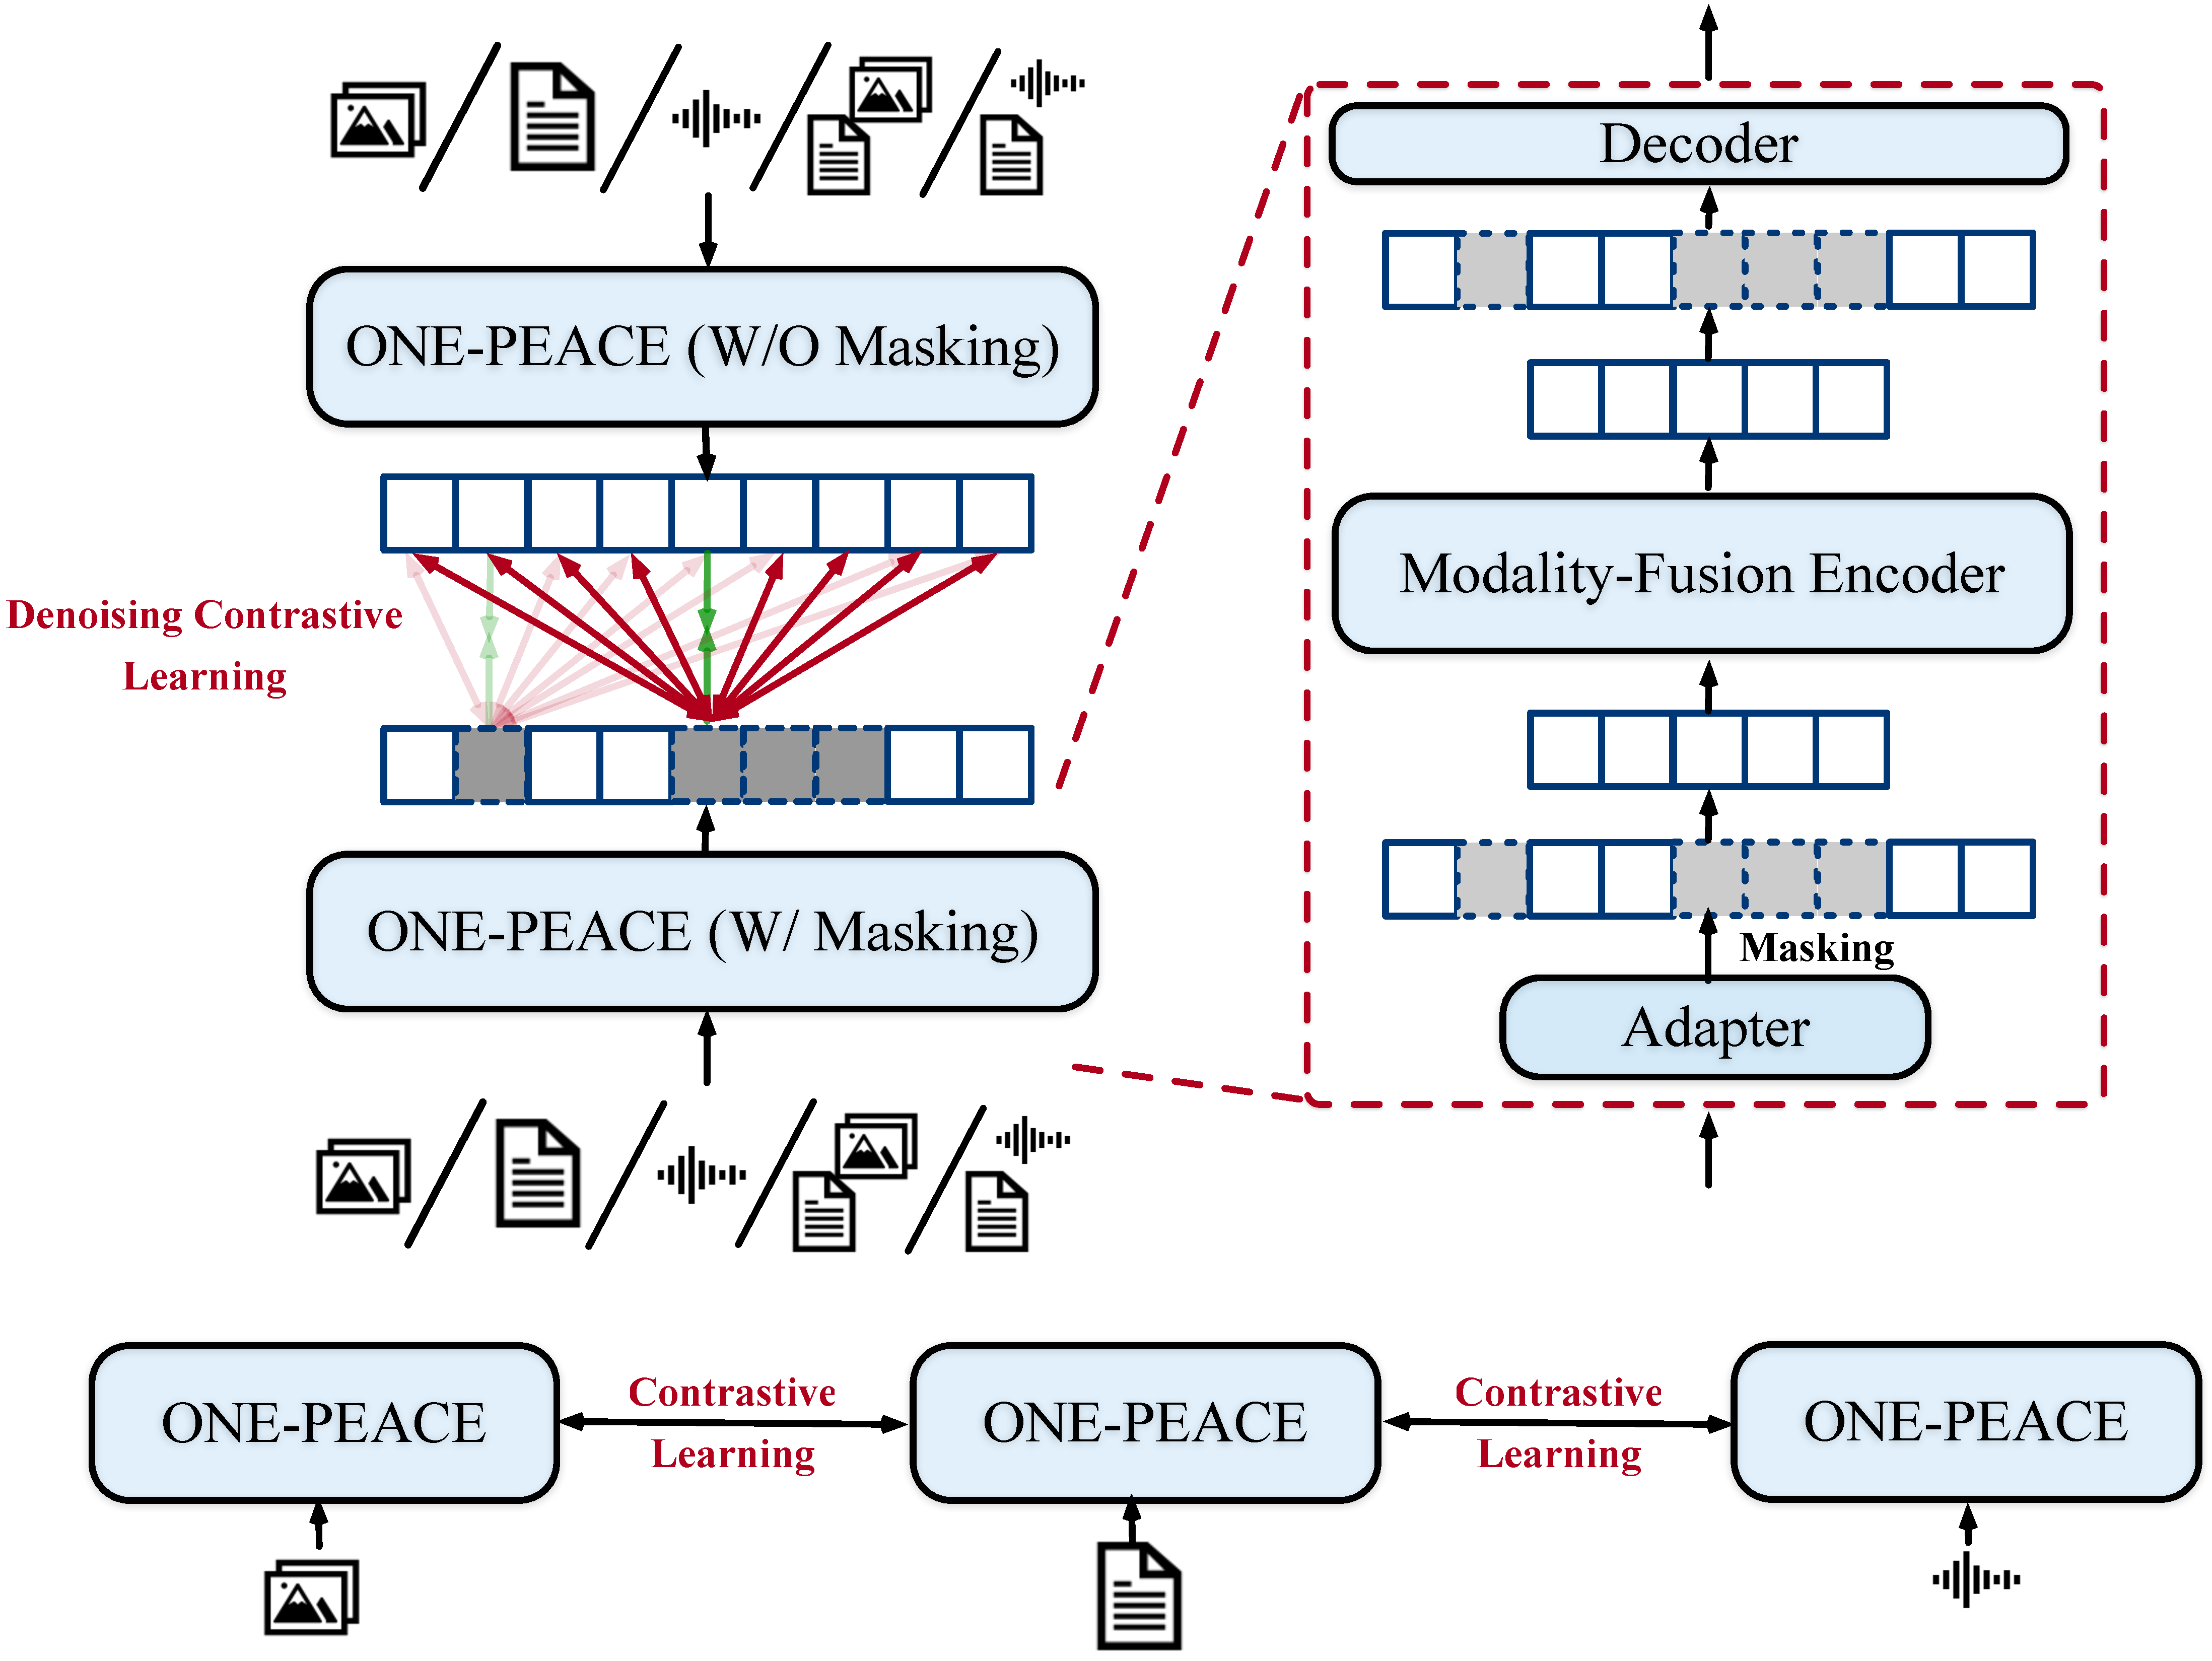
\includegraphics[width=0.8\linewidth]{pic/pretraining_tasks.pdf}
    \caption{\textbf{The pretraining tasks of \onepeace.} Intra-modal denoising contrastive learning encourages the features of the masked units (e.g., image patches or text tokens) close to the positive units (indicated by the green lines) and get away from the negative units (indicated by the red lines). Note that we compute the cross-modal contrastive loss by gathering negative features from all GPU devices, while the denoising contrastive loss is computed on the local batch.}
    \label{fig:loss}
\end{figure*}

\subsection{Tasks}
The pretraining tasks of \onepeace include cross-modal contrastive learning and intra-modal denoising contrastive learning. 
Cross-modal contrastive learning endows the model with cross-modal retrieval capability, while intra-modal denoising contrastive learning enables the model to achieve superior fine-tuning performance in downstream tasks. 
An illustration of the pretraining tasks is shown in Figure~\ref{fig:loss}.

\paragraph{Cross-Modal Contrastive Learning.}
% We perform cross-modal contrastive learning to align the semantic space of vision, language, and audio.
% It contains both vision-language contrastive learning and audio-language contrastive learning.
% Given an image-text pair $\left(I, T\right)$, we use the V-Branch and L-Branch to extract the image features and text features, respectively.
% We regard the final output of vision class token and language class token as the global representations.
% Followed by a linear projection and normalization, we obtain the image embedding $\bm{s}^V$ and language embedding $\bm{s}^L$.
% Similarly, given an audio-text pair $\left( A, T'\right)$, we use the A-Branch and L-Branch to obtain the audio embedding $\bm{s}^A$ and language embedding $\bm{s}^{L'}$.
% The contrastive loss functions are shown below:

% \begin{equation}
% \mathcal{L}_{CL-VL} = -\frac{1}{2N}\sum_{i=1}^{N}({\rm log}\frac{{\rm exp}(\bm{s}_i^{V}\bm{s}_i^{L}/\sigma)}{\sum_{j=1}^{N}{\rm exp}(\bm{s}_i^V\bm{s}_j^L/\sigma)} + {\rm log}\frac{{\rm exp}(\bm{s}_i^{V}\bm{s}_i^{L}/\sigma)}{\sum_{j=1}^{N}{\rm exp}(\bm{s}_j^V\bm{s}_i^L/\sigma)}),
% \end{equation}

% \begin{equation}
% \mathcal{L}_{CL-AL} = -\frac{1}{2N}\sum_{i=1}^{N}({\rm log}\frac{{\rm exp}(\bm{s}_i^A\bm{s}_i^{L'}/\sigma)}{\sum_{j=1}^{N}{\rm exp}(\bm{s}_i^A\bm{s}_j^{L'}/\sigma)} + {\rm log}\frac{{\rm exp}(\bm{s}_i^A\bm{s}_i^{L'}/\sigma)}{\sum_{j=1}^{N}{\rm exp}(\bm{s}_j^A\bm{s}_i^{L'}/\sigma)}),
% \end{equation}

% where $\mathcal{L}_{VL}$ and $\mathcal{L}_{AL}$ refer to the vision-language contrastive loss and audio-language contrastive loss, respectively. $N$ is the batch size, $i,j$ are indexes within the batch, and $\sigma$ is a learnable temperature parameter (initialized to $0.07$).

Cross-modal contrastive learning is a widely-used pretraining task that effectively aligns the semantic spaces of different modalities. 
The key idea of this method is to maximize the similarity of related sample pairs across different modalities while minimizing the similarity of unrelated sample pairs.
Given a sample pair $(S^1, S^2)$ of arbitrary modalities (e.g., image-text pair or audio-text pair), we extract their features using the corresponding branches of \onepeace.
The outputs of the special tokens (e.g., vision class token or language class token) are regarded as global representations. Followed by a linear projection and normalization, we obtain the final representations $\bm{s}^1$ and $\bm{s}^2$. The loss function is shown below:

\begin{equation}
\mathcal{L}_{CL} = -\frac{1}{2N}\sum_{i=1}^{N}({\rm log}\frac{{\rm exp}(\bm{s}_i^{1}\bm{s}_i^{2}/\sigma)}{\sum_{j=1}^{N}{\rm exp}(\bm{s}_i^1\bm{s}_j^2/\sigma)} + {\rm log}\frac{{\rm exp}(\bm{s}_i^{1}\bm{s}_i^{2}/\sigma)}{\sum_{j=1}^{N}{\rm exp}(\bm{s}_j^1\bm{s}_i^2/\sigma)}),
\end{equation}

where $N$ is the batch size, $i,j$ are indexes within the batch, and $\sigma$ is a learnable temperature parameter (initialized to $0.07$). Following previous works~\cite{clip,align}, the cross-modal contrastive loss is computed by gathering negative features from all GPU devices.
We apply cross-modal contrastive learning to image-text pairs and audio-text pairs, denoted by $\mathcal{L}_{CL-VL}$ and $\mathcal{L}_{CL-AL}$ respectively.
% Despite not training on image-audio pairs, the semantic space between vision and audio is still aligned by using language as the anchor.

\paragraph{Intra-Modal Denoising Contrastive Learning.}
% Inter-modal contrastive learning endows the model with powerful zero-shot retrieval capabilities. However, since inter-modal contrastive learning pays more attention to the global representation of the samples, it tends to make the model ignore the internal details inside each sample. 

% We strive to maintain the cross-modal retrieval capability of our model while achieving excellent performance when transferred to downstream tasks. 
% Initially, we considered combining cross-modal contrastive learning with the masked prediction task~\cite{bert,beit,mae}. 
% However, we found that directly integrating the masked prediction task would compromise the model's cross-modal retrieval ability. 
% To address this issue, we formulated the masked prediction task as a masked intra-modality contrastive learning task. 
% Our experiments indicate that masked intra-modality contrastive learning is highly compatible with cross-modal contrastive learning. 
% We subsequently apply masked intra-modality contrastive learning to each modality.

Cross-modal contrastive learning mainly focuses on aligning features between different modalities. 
However, it lacks emphasis on the learning of fine-grained details within modalities, leading to suboptimal performance in downstream tasks~\cite{fd-clip}. 
To address this issue, we further introduce intra-modal denoising contrastive learning to train \onepeace\footnote{Intra-modal denoising contrastive learning is similar to \cite{conmim}, but extends to more modalities.}.
Intra-modal denoising contrastive learning can be viewed as a combination of masked prediction and contrastive learning, where we perform contrastive loss between the fine-grained masked features and visible features, such as image patches, text tokens, or audio waveform features.

Given a sample of arbitrary modalities, we first encode it into an embedding sequence through the corresponding modality adapter.
Then, we randomly mask some units (e.g., text tokens or image patches) within the sequence.
Following~\cite{mae}, we only input the unmasked units to the modality fusion encoder to reduce computation costs and save memory.
The encoded unmasked features are concatenated with the learnable mask tokens and fed to a lightweight Transformer decoder, which generates the masked features.
We also use the \onepeace model to encode the raw input sample into target features without masking.
Finally, we perform the contrastive loss between the masked features and target features, the loss function is shown below:

\begin{equation}
\label{eq:mcl}
\mathcal{L}_{DCL} = -\frac{1}{N\hat{N}}\sum_{i=1}^{N}\sum_{j=1}^{\hat{N}}{\rm log}\frac{{\rm exp}(\bm{\hat{h}}_{ij} \cdot {\rm sg}(\bm{h}_{ij})/\tau)}{\sum_{m=1}^{N}\sum_{n=1}^{N}{\rm exp}(\bm{\hat{h}}_{ij}  \cdot {\rm sg}(\bm{h}_{mn})/\tau)},
\end{equation}

Where $\bm{\hat{h}}_{ij}$ is the representation of the masked unit, $\bm{h}_{ij}$ is the representation of the target unit, $\text{sg}(\cdot)$ is the stop gradient operation. $\hat{N}$ is the number of masked units within a sample, $N$ is the number of whole units within a sample. $\tau$ is a constant temperature value, we set it to $0.4$. 
This loss not only encourages the masked units close to the positive units but also gets away from the negative units.
As a result, each unit acquires a unique semantic meaning, which makes the model better transfer to downstream tasks~\cite{fd-clip}.

We apply intra-modal denoising contrastive learning to $5$ types of data: image, audio, text, image-text pairs, and audio-text pairs.
For image, we randomly mask $75\%$ patches, and the loss function used for this type of data is denoted by $\mathcal{L}_{DCL-V}$.
For audio, we sample $p=0.11$ of all time-steps to be starting indices and mask the subsequent $5$ time-steps, and the loss function is denoted by $\mathcal{L}_{DCL-A}$.
For text, we randomly mask $15\%$ tokens of the text sequence, and the loss function is denoted by $\mathcal{L}_{DCL-L}$.
For image-text pairs, we randomly mask $68.75\%$ patches of the image and $40\%$ tokens of the text. The unmasked patches and tokens are concatenated together and encoded as masked features.
The original image patches and text tokens are also concatenated together and encoded as target features.
We then perform contrastive loss on the image patches and text tokens respectively, the average of these two
losses is denoted by $\mathcal{L}_{DCL-VL}$.
For audio-text pairs, we randomly mask $45\%$ time-steps of the audio waveform and $40\%$ tokens of the text. 
The loss is similar to the above one, we denote it by $\mathcal{L}_{DCL-AL}$.

\subsection{Training}
\label{sec:two_stage_pretraining}
The overall pretraining process of \onepeace is divided into two stages: vision-language pretraining and audio-language pretraining.
At the vision-language pretraining stage, the model trains on image-text pairs and only updates parameters that are relevant to vision and language modalities.
For each image-text pair, we not only utilize them to calculate $\mathcal{L}_{CL-VL}$ and $\mathcal{L}_{DCL-VL}$, but also separately using the image and text to calculate $\mathcal{L}_{DCL-V}$ and $\mathcal{L}_{DCL-L}$ respectively.
The loss function at this stage is shown below:

\begin{equation}
\mathcal{L}_{VL} = \mathcal{L}_{CL-VL} + 1.0*\mathcal{L}_{DCL-V} + 0.5*\mathcal{L}_{DCL-L} + 1.0*\mathcal{L}_{DCL-VL}
\end{equation}

At the audio-language pretraining stage, the model trains on audio-text pairs, and we only update A-Adapter, A-FFNs, and other audio-related parameters. 
The remaining parameters including self-attention layers are totally frozen.
Despite not training on image-audio pairs, the semantic space between vision and audio is still aligned by using language as the anchor.
The loss function at the audio-language pretraining stage is shown below:

\begin{equation}
\mathcal{L}_{AL} = \mathcal{L}_{CL-AL} + 1.0*\mathcal{L}_{DCL-A} + 1.0*\mathcal{L}_{DCL-AL}
\end{equation}

% Although \onepeace didn't train on image-audio pairs, the semantic space between vision and audio is still aligned by using language as the anchor.

\section{Pretraining Details}
\begin{table*}[t]
\centering
\tablestyle{4pt}{1.2}
\begin{tabular}{cccccccccccc}
  \multirow{2}{*}{\#Layers}
  & \multirow{2}{*}{\bf \tabincell{c}{\scriptsize Hidden \\ \scriptsize Size}}
  & \multirow{2}{*}{\bf \tabincell{c}{\scriptsize Intermediate \\ \scriptsize Size}}
  & \multirow{2}{*}{\bf \tabincell{c}{\scriptsize Attention \\ \scriptsize Size}}
  & \multicolumn{8}{c}{\textbf{\#Parameters}}
  \\
  \cmidrule(lr){5-12}
  &
  &
  &
  & \textbf{\scriptsize V-Adapter}
  & \textbf{\scriptsize A-Adapter}
  & \textbf{\scriptsize L-Adapter}
  & \textbf{\scriptsize V-FFN}
  & \textbf{\scriptsize A-FFN}
  & \textbf{\scriptsize L-FFN}
  & \textbf{\scriptsize Shared Attention}
  & \textbf{\scriptsize Total}
  \\
  \shline
  40
  & 1536
  & 6144
  & 24
  & 3.4M
  & 19M
  & 78M
  & 1.15B
  & 1.15B
  & 1.15B
  & 378M
  & 4B
  \\
\end{tabular}
% \vskip 0.15in
\caption{\textbf{Detailed hyperparameters of \onepeace model configuration.}}
\label{tb:model_configuration}
\end{table*}

\paragraph{Pretraining Datasets.}
The pretraining datasets of \onepeace are divided into two parts: image-text pairs and audio-text pairs. 
For image-text pairs, we use LAION-2B~\cite{laion5b}, a dataset obtained by web crawling.
For audio-text pairs, we collect a large amount of open-source environmental sound datasets.
To ensure reproducibility, all pretraining datasets are publicly available.
We provide more details about the pretraining datasets in Appendix~\ref{app:audio_text_data_details}.

% \paragraph{Pretraining Datasets}
% Our pretraining datasets are divided into two parts: image-text pairs and audio-text pairs. 
% For image-text pairs, we use LAION-2B, a pre-training dataset obtained by web crawling that may contain some noisy pairs. To improve the data quality, we apply several pre-processing steps, including removing images with an aspect ratio greater than 3.5, removing images with the shortest side less than 128, and removing images with a clip score less than 0.3. We also remove texts containing non-English or emoji characters, as well as texts with lengths less than 3 or greater than 512. After these steps, we retain about 1.5 billion image-text pairs.

% For audio-text pairs, we collect a large amount of open-source environmental sound datasets and perform simple cleaning on the data, which involves removing samples with text lengths less than 3 or greater than 512, as well as texts containing non-English or emoji characters. Ultimately, we preserve about 2.4 million audio-text pairs, with a total duration of around 8,000 hours. More information about the environmental sound data can be found in Appendix~\ref{app:audio_text_data_details}

\paragraph{Pretraining Settings.}
\begin{table*}[t]
\centering
\normaltablestyle{6pt}{1.2}
\begin{tabular}{*l| ^c ^c ^c| ^c}
Method                                 & Enc. \#Params & Patch Size & Image size & Top-1 acc \\
\shline
FD-SwinV2-G~\cite{wei2022contrastive}  & 3.0B  & $16\times16$ & 336$^2$    & 89.4 \\
InternImage~\cite{wang2022internimage} & 1.08B & $16\times16$ & 640$^2$    & 89.2 \\
BEiT-3~\cite{beit3}                    & 1.01B & $14\times14$ & 336$^2$    & 89.6 \\
EVA~\cite{eva}                         & 1.01B & $14\times14$ & 560$^2$    & 89.7 \\
\hline
\modelname                             & 1.52B & $16\times16$ & 384$^2$    & 89.6 \\
\modelname                             & 1.52B & $16\times16$ & 512$^2$    & \textbf{89.8}
\\
\hline
\multicolumn{5}{l}{\rowstyle{\color{dt}}\textit{methods using extra privately collected data:}}
\\
\hline
\rowstyle{\color{dt}}RevCol-H~\cite{cai2022reversible}      & \color{dt}2.16B & - & 640$^2$    & 90.0 \\
\rowstyle{\color{dt}}ViT-G~\cite{modelsoups}      & \color{dt}1.84B & $14\times14$ & 518$^2$    & 90.5 \\
\rowstyle{\color{dt}}Model Soups~\cite{modelsoups}      & \color{dt}1.84B & $14\times14$ & 500$^2$    & 90.9 \\
\rowstyle{\color{dt}}CoCa~\cite{coca}      & \color{dt}1.01B & $18\times18$ & 576$^2$    & 91.0 \\
\end{tabular}
\caption{\textbf{System-level comparisons of image classification with the leading results on ImageNet-1k.} RevCol~\cite{cai2022reversible} is pretrained on a privately collected 168-million-image dataset. ViT-G~\cite{modelsoups} and Model Soups~\cite{modelsoups} are pretrained on JFT-3B~\cite{jft} with supervision. CoCa~\cite{coca} uses JFT-3B~\cite{jft} and ALIGN~\cite{align} datasets for pretraining. \onepeace achieves state-of-the-art results using the publicly available dataset with less token length.}
\label{tb:inet1k}
\end{table*}
\onepeace is a giant-size model with $4$B parameters. We list the detailed hyper-parameters in Table~\ref{tb:model_configuration}. 
During pretraining, we introduce a lightweight Transformer decoder to recover the masked units from the visible units. The decoder is similar to the modality-fusion encoder, each block of it also consists of a shared self-attention layer and three modality FFNs.
It has $2$ layers with $768$ hidden size, $2048$ intermediate size, and $12$ attention heads.
The model weights of \onepeace are randomly initialized at the beginning, except for the audio feature extractor of A-adapter, for which we use the weights of WavLM's feature extractor~\cite{wavlm} for initialization. 
We find that incorporating WavLM's feature extractor significantly improves the model performance.
% We find that a randomly initialized feature extractor leads to overfitting, whereas incorporating the weights from WavLM's feature extractor~\cite{wavlm} significantly mitigated this problem and improves the model performance.
More details about the pretraining settings are provided in Appendix~\ref{app:pretraining_hyperparameters}.

\paragraph{Training Acceleration.}
We introduce several model acceleration and memory optimization techniques to accelerate the training.
Firstly, we use the memory-efficient attention technique~\cite{memory_efficient_attn,flash_attn} implemented in the xformers library\footnote{\url{https://github.com/facebookresearch/xformers}} to improve training speed.
Secondly, we use the gradient checkpointing technique~\cite{checkpointing} to save memory, which allows us to train the model with a larger batch size.
Furthermore, we replace the layer normalization with Fused LayerNorm implemented in the Flash Attention library\footnote{\url{https://github.com/HazyResearch/flash-attention}}, and leverage nvFuser\footnote{\url{https://pytorch.org/blog/introducing-nvfuser-a-deep-learning-compiler-for-pytorch}} to fuse the operations of dropout, LayerScale, stochastic depth, and residual summing, which can bring additional speed improvements.
To improve the training speed and prevent gradient overflow issues, we adopt Bfloat16 precision to train \onepeace.